\documentclass[12pt,a4paper]{report}

%
% PACKAGES AND STYLES
%

% 
% Language and encoding
%
%\usepackage{mathtext}
%\usepackage[T2A]{fontenc}
\usepackage[utf8]{inputenc}
\usepackage[english,russian]{babel}
\usepackage{mmap}

%
% Colors
%
\usepackage[usenames]{color}
\usepackage{color}
\usepackage{colortbl}

%
% Symbols
%
\usepackage{amssymb}
\usepackage{MnSymbol}

%
% Units
%
%\usepackage[binary-units=true]{siunitx}
\newcommand{\km}{\mathrm{~\text{км}}}
\newcommand{\m}{\mathrm{~\text{м}}}
\newcommand{\s}{\mathrm{~\text{с}}}
\newcommand{\mps}{\m \s ^{-1}}
\newcommand{\pers}{\s ^{-1}}
\newcommand{\K}{\mathrm{~\text{К}}}
\newcommand{\Kpkm}{\K\km ^{-1}}
\newcommand{\hpa}{\mathrm{~\text{гПа}}}
\newcommand{\J}{\mathrm{~\text{Дж}}}
\newcommand{\Jpm}{\J \m ^{-3}}

%
% Paper size and margins
%
\usepackage{vmargin}
\setmarginsrb{2.5cm}{1cm}{2.5cm}{2cm}{0cm}{0cm}{0cm}{1.5cm}

%
% Page style
%
\usepackage{fancyhdr}
\setlength{\headheight}{16pt}
\newcommand{\changefont}{%
    \fontsize{9}{11}\selectfont
}
\fancyhf{}
\fancyhead[RO]{\changefont \slshape \rightmark} %section
\fancyhead[LO]{\changefont \slshape \leftmark} %chapter
\fancyfoot[C]{\changefont \thepage} %footer
\setlength{\headsep}{0.2in}
\pagestyle{fancy}

%
% Indenting
%
\usepackage{indentfirst}
\setlength{\parindent}{1cm}
\setlength{\parskip}{0.5cm}

%
% References
%
\usepackage{natbib}

%
% Hyperlinks
%
\usepackage[linktocpage=true,plainpages=false,pdfpagelabels=false]{hyperref}
\definecolor{linkcolor}{rgb}{0.1,0,0.9}
\definecolor{citecolor}{rgb}{0,0,0.9}
\definecolor{urlcolor}{rgb}{0,0,1}
\hypersetup{
    colorlinks, linkcolor={linkcolor},
    citecolor={citecolor}, urlcolor={urlcolor}
}

\bibliographystyle{plainnat}
% Bibliography: set article volume number in bold font
%\DeclareFieldFormat
%  [article]
%  {volume}{\textbf{#1}}
%\renewcommand\nameyeardelim{, }

%\usepackage{showkeys} % show labels

\newcommand{\figref}[1]{\mbox{Figure~\ref{#1}}}
\newcommand{\tabref}[1]{\mbox{Table~\ref{#1}}}
\newcommand{\secref}[1]{\mbox{Section~\ref{#1}}}
\newcommand{\chpref}[1]{\mbox{Chapter~\ref{#1}}}
\newcommand{\appref}[1]{\mbox{Appendix~\ref{#1}}}
\newcommand{\eqnref}[1]{\mbox{Eq.~(\ref{#1})}}
\newcommand{\listref}[1]{\mbox{Listing~(\ref{#1})}}

%
% Lists
%
\usepackage[shortlabels]{enumitem}

\newenvironment{sqlist}[1][\enskip$\filledsquare$]
        {\begin{itemize}[#1]}
        {\end{itemize}}

% New math commands
% differential d, from http://tex.stackexchange.com/a/60546/586
\newcommand*\diff{\mathop{}\!\mathrm{d}}
\newcommand\mean[1]{\overline{#1}}
\newcommand{\PDt}[2]{\partial #1/\partial #2}

%
% Tables
%
\usepackage{booktabs}
%\usepackage{tabularx}
\usepackage{tabu}
\usepackage{longtable}

%
% Figures
%
\usepackage{wrapfig}
\usepackage[font=small,textfont=it,labelfont=bf]{caption}
%\captionsetup[figure]{labelfont=bf}
\usepackage{tikz}
\usepackage{pgfplots}
\usetikzlibrary{calc}

%
% Equations
%
\usepackage{cool}


\begin{document}
\setcounter{chapter}{3}
\chapter{Результаты}
Данный раздел посвящен обзору результатов численного моделирования, постановка которых описана выше. Раздел построен следующим образом: сначала рассматривается контрольный эксперимент, а именно структура, динамика и энергетика вихря. Затем аналогичным образом описывается эксперимент со включенной параметризацией микрофизики, и оценивается чувствительность вихря к начальному содержанию влаги в атмосфере.

\begin{wrapfigure}{L}{0.5\textwidth}
\begin{center}
\includegraphics[scale=0.25]{{./chapters/figures_results/pt_dev_z.x26-x76.y26-y76.ilev01.020000_}.jpg}
\end{center}
\caption{Поле отклонений температуры ($\theta'$) при инициализации возмущения (2 ч. модельного времени)}
\label{fig:initanom}
\end{wrapfigure}

Влияние остальных факторов на динамику мезоциклона рассматривается с точки зрения таких интегральных характеристик, как кинетическая энергия, максимальная завихренность, минимальное приземное давление. Для интерпретации различий в результатах оценочных экспериментов привлекается анализ пространственной структуры метеополей.

Полярный мезоциклон в каждом эксперименте развивался с разной скоростью, и продолжительность экспериментов составляет 1-3 сут. Трехмерные поля в каждый момент времени интерполируются на регулярную сетку с горизонтальным разрешением, соответствующим разрешению модели. В экспериментах без фонового потока горизонтальные разрезы сфокусированы на район развития вихря (обычно $200\times 200\km$ в центре области). По вертикали данные интерполируются на регулярную сетку с шагом $500\m$ для удобства последующего постпроцессинга. В некоторых экспериментах также используется интерполяция на изобарические поверхности от $1000$ до $250\hpa$ с шагом $50\hpa$.

\section{Контрольный эксперимент}
\subsection{Начальная стадия развития вихря}
Начнем с рассмотрения момента инициализации температурной аномалии. Ее форма и начальная амплитуда видна на рис. \ref{fig:initanom}.

Появление источника тепла в атмосфере, находящейся в равновесии, ставит проблему реакции атмосферы и достижения нового баланса через механизм приспособления. Этот вопрос впервые был развит Лэмбом \citep{RT2003}, который изучал особенности волн, излучаемых в процессе гидростатического приспособления. Позднее эта проблема была обобщена как ответ устойчиво стратифицированной атмосферы на вертикально ограниченный, но горизонтально однородный источник тепла. Один из интересных результатов, полученных в работе \citep{Bannon1995}, заключаются в том, что если источник тепла горизонтально однороден, то слои воздуха ниже источника не смещаются относительно начального положения. Слои же воздуха выше источника одинаково подняты вверх. Источник нагрева в нижней тропосфере влияет на распределение давления во всей толще атмосферы выше него. Для оценки высоты, на которую распространяется влияние нагрева снизу в работе \citep{Bannon1995} было введено понятие вертикальный масштаб возмущения применительно к изотермической атмосфере. При этом в атмосфере с реалистичной структурой этот масштаб несильно отличается от такового для изотермической атмосферы. Так как распределение давления больше всего меняется на верхней границе нагретого слоя, и ответ поля давления на источник тепла убывает с высотой экспоненциально, в случае нагрева нижних слоев тропосферы эффект будет проявляться главным образом в тропосфере.

Более интересно для реальной атмосферы рассмотреть проблему Лэмба для случая неоднородного источника тепла. Например, если взять источник тепла определенного радиуса, то он будет излучать не только вертикально распространяющийся горизонтальный волновой фронт, но и сферический волновой фронт, распространяющийся от внешнего радиуса аномалии горизонтально и вертикально. 

\begin{wrapfigure}{R}{0.5\textwidth}
\begin{center}
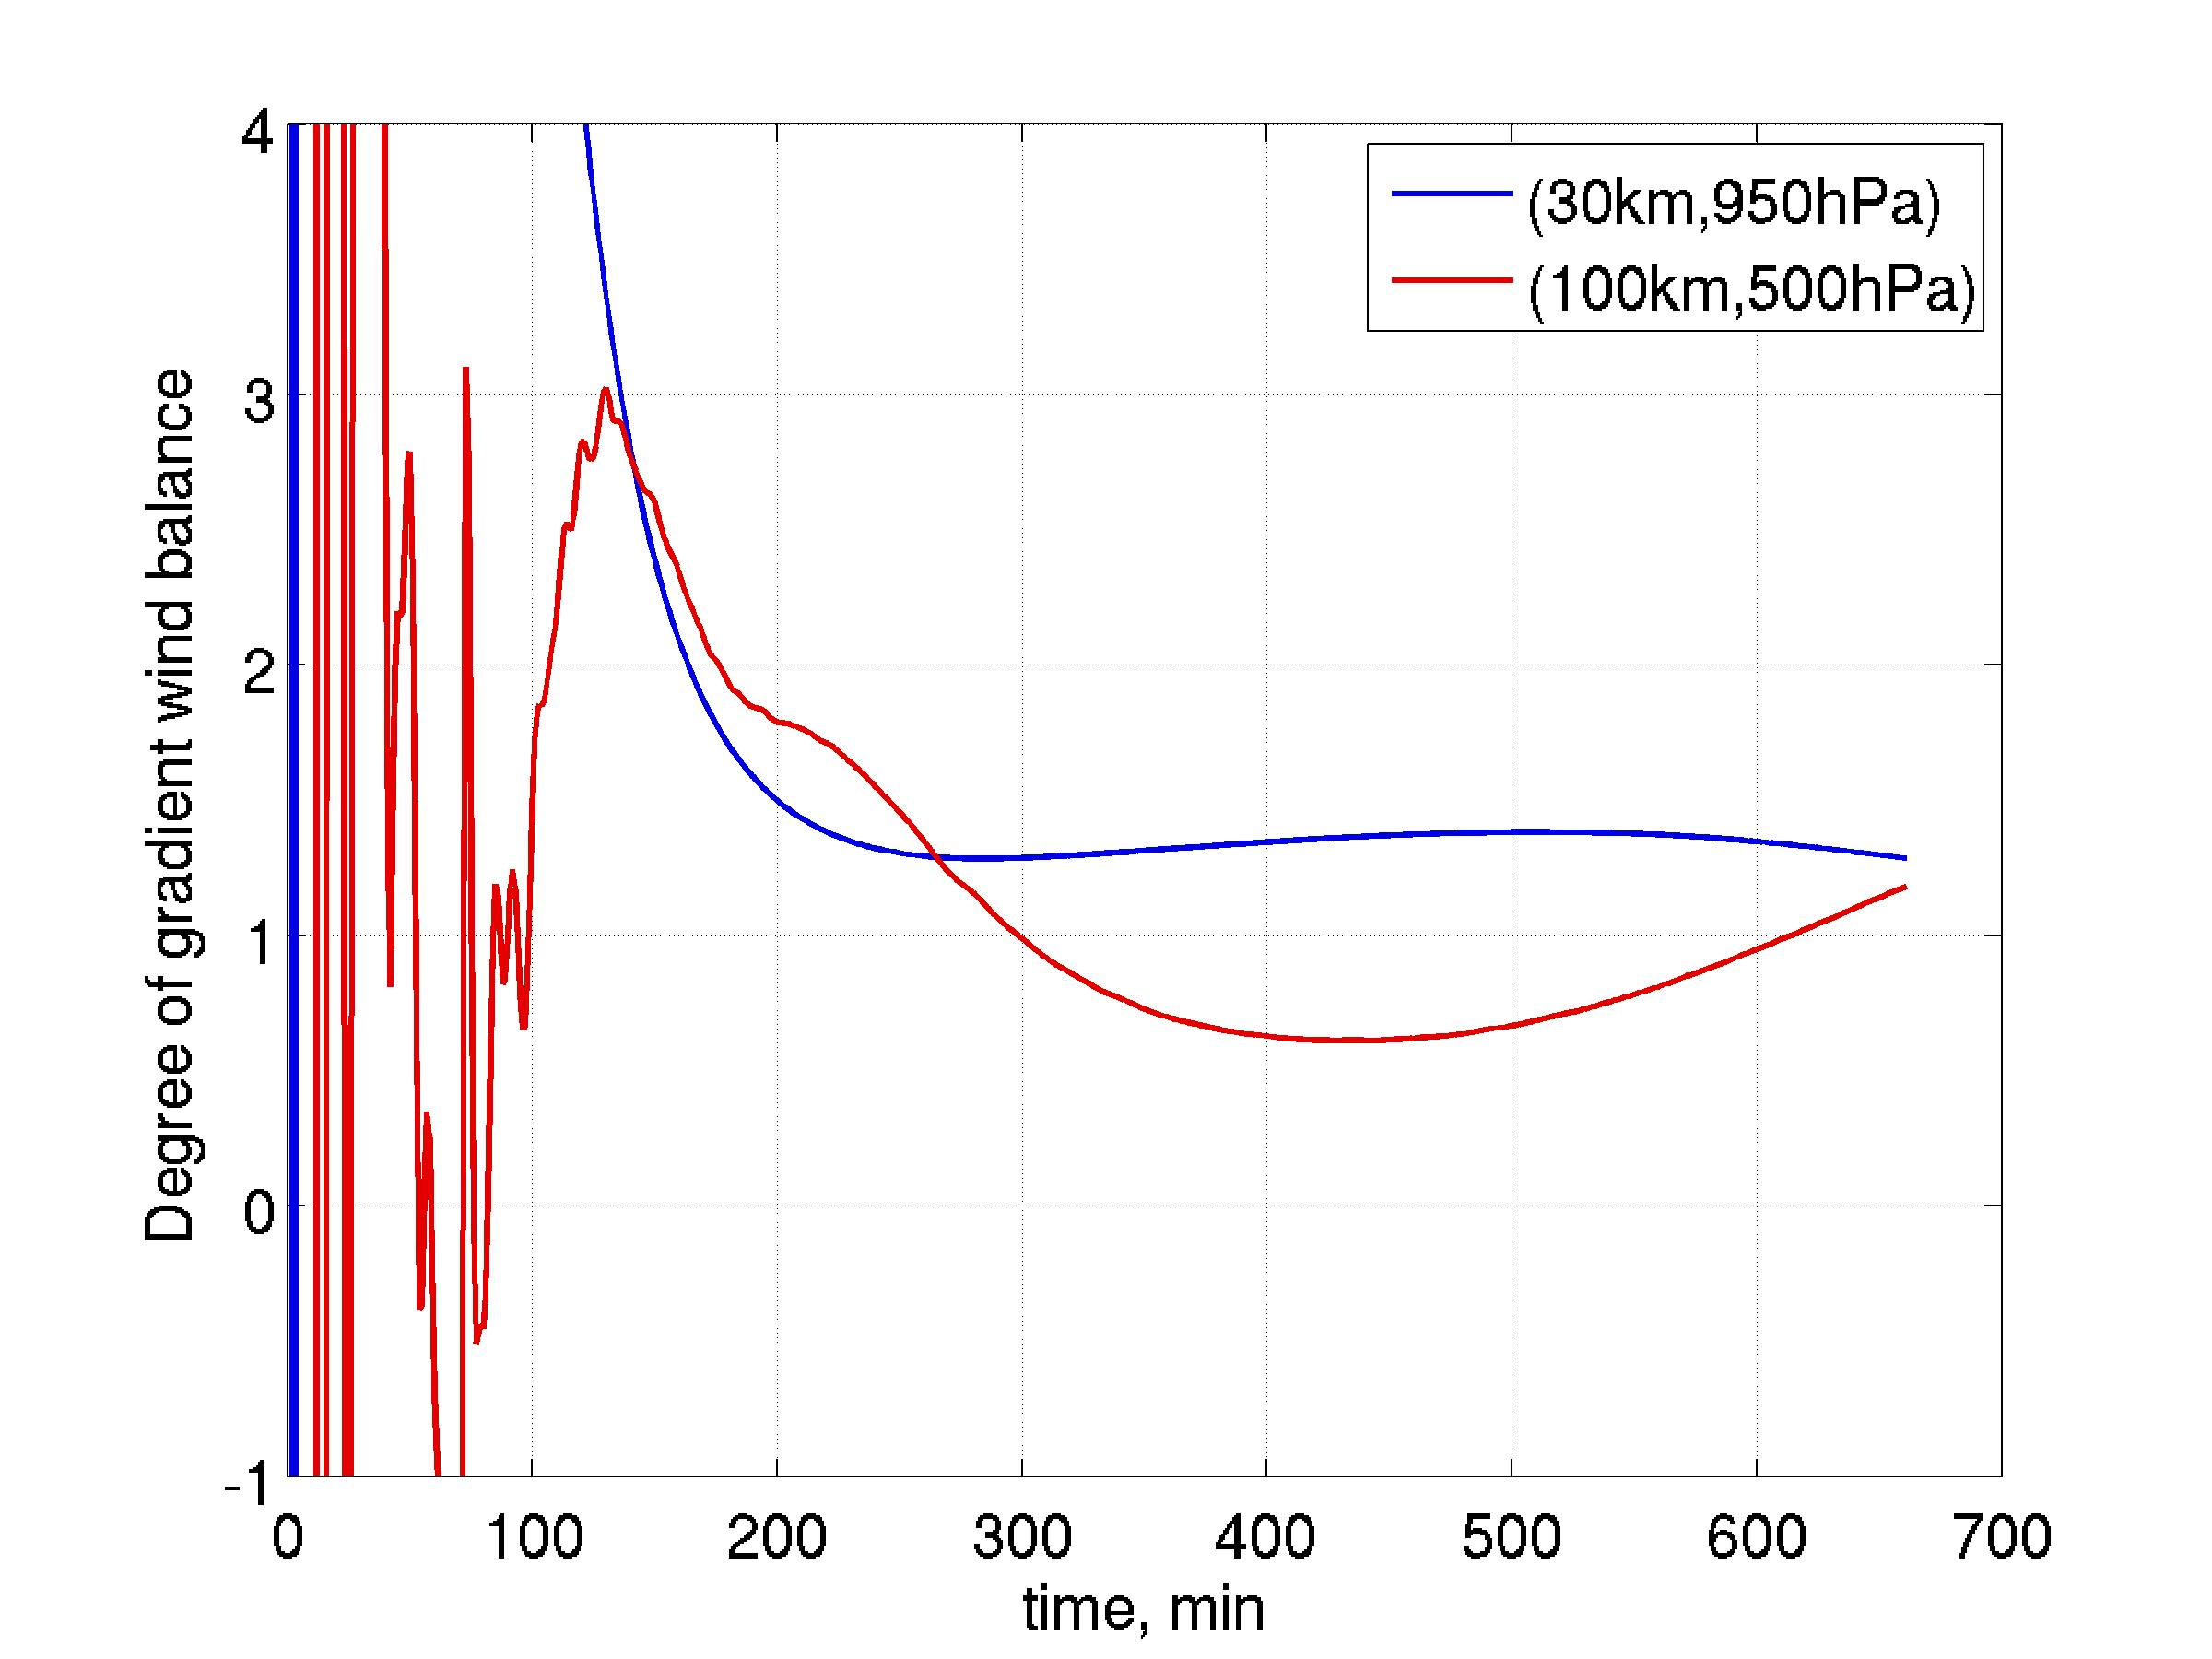
\includegraphics[scale=0.09]{{./chapters/figures_results/ctrl_grwindbal2p}.jpg}
\end{center}
\caption{Величина градиентного баланса $\pderiv{\phi'}{r}/\left(v^2_t/r+fv_t\right)$ как функция времени с момента инициализации возмущения: при $r=30\km, p=950\hpa$ (синяя кривая) и при $r=100\km, p=500\hpa$ (красная кривая). Градиентный баланс достигается, когда кривые приближаются к $1$.}
\label{fig:grwindbal}
\end{wrapfigure} 

Подобный процесс наблюдается в начале каждого эксперимента данной работы. Ввиду того, что нагрев в районе аномалии происходит не мгновенно, а в течение конечного отрезка времени, как и бывает в реальной атмосфере,  фронт излучаемых волн прослеживается слабее. Тем не менее, результат качественно совпадает идеализированными экспериментами \citep{RT2003}. Вертикальный барический градиент находится почти в гидростатическом балансе с силой плавучести, а горизонтальный создает циклоническую циркуляцию. Такая циркуляция возникает в устойчиво стратифицированной атмосфере, и источник энергии в виде конвективной доступной потенциальной энергии (CAPE) не является необходимым. При остановке подачи тепла не вращающаяся атмосфера постепенно придет к состоянию покоя. Однако это не так, если атмосфера испытывает вращение, что подтверждается в наших экспериментах \ref{sec:res:nohle}.

Начальная куполообразная аномалия приводит к возникновению в нижних слоях атмосферы горизонтального градиента давления, который создает конвергенцию массы в центре области. В результате под влиянием силы Кориолиса возникают инерционно-гравитационные волны, в то время как возникновение звуковых волн невозможно ввиду разрешения сетки модели (\citep{MillerWhite1984,MirandaPhD}). Путем излучения инерционно-гравитационных волн происходит приспособление атмосферы к градиентному балансу (\ref{fig:grwindbal}).

Вертикальный разрез вертикальной скорости \ref{} дает представление о распространении гравитационных волн в ответ на температурное возмущение. Рисунок схож с результатами линейной теории \citep{Lin2007}, однако более правдоподобен из-за нелинейности процессов и интерференции волн в реальной атмосфере. При задании неоднородного фонового профиля стратификации области подъема и нисхождения воздуха, очевидно, будут иметь несимметричную форму.

Несмотря на четко различимые в начале моделирования волны, их влияние мало: аномалия потенциального вихря, определяющая циркуляцию в атмосфере, остается на месте, где она была изначально помещена. На рис. \ref{fig:grwindbal} частота проходящих через выбранные точки волн уменьшается, то есть волны с меньшими частотами остаются в вихре, а более высокочастотные волны распространяются наружу. Другими словами, возмущение потенциального вихря не переносится вместе с инерционно-гравитационными волнами \citep{RT2003}. Влияние волн, созданных начальным дисбалансом в атмосфере пренебрежимо мало по сравнению с "равновесной" частью движения, которое связано через принцип обратимости с распределением потенциального вихря.

Равновесная часть движения формируется сразу после инициализации температурной аномалии. Подтверждением того, что наибольший вклад в развитие циркуляции имеет конвергенция массы, служит анализ уравнения завихренности \citep{Bluestein1992I} для $f$-плоскости (слагаемые, содержащие параметр $\beta=\partial f/ \partial y$ и силу трения опущены):
\begin{equation}
\label{eq:vorttend}
\pderiv{\zeta}{t}=-\vec{v}\cdot \nabla_z \zeta - w\pderiv{\zeta}{z} - (\zeta + f)\left(\pderiv{u}{x}+\pderiv{v}{y}\right) 
+ \vec{k}\cdot\left(\pderiv{\vec{v}}{z}\times\nabla w\right) + \vec{k}\cdot\left(\nabla p \times \nabla\alpha \right),
\end{equation}
где $\zeta$ – вертикальная компонента вектора вихря скорости (завихренность), $\vec{v}=(u,v,w)$ - вектор скорости, $\alpha=1/\rho$ - удельный объем. Рассмотрим состояние эксперимента в 3 час модельного времени – в момент, когда аномалия только что была инициализирована. На рис. \ref{} представлены пространственное распределение компонент, входящих в правую часть ур. \ref{eq:vorttend}. Данные осреднены по вертикали в слое от $0$ до $1000\m$, в котором в течение всего времени наблюдаются наибольшие значения градиентов скорости.

Нетрудно заметить, что содержащее горизонтальную дивергенцию слагаемое (слагаемое растяжения) имеет наибольшие значения, причем его экстремум совпадает с экстремумом тенденции завихренности и они близки по значению. Недостающую часть тенденции вихря составляет вертикальная адвекция. Величина завихренности уже достаточно велика в данный момент (приблизительно в 2 раза меньше, чем значение параметра Кориолиса), а скорость ее роста говорит о том, что меньше, чем через час значения удвоятся. Бароклинное слагаемое (ур. \ref{eq:vorttend}, последнее слагаемое) – произведение градиентов давления и плотности – имеет значения на 3-4 порядка меньшие остальных членов, и это соотношение сохраняется в течение всего эксперимента. Поэтому далее бароклинное слагаемое рассматриваться не будет.

\subsection{Эволюция вихря}
Общую картину динамики вихря дают графики изменения максимума завихренности в нижней тропосфере и минимума аномалии приземного давления (\ref{}). Более детально структура вихря будет рассмотрена в следующем разделе. В контрольном эксперименте не удалось получить устойчивый вихрь: интенсивность начального возмущение с возрастающей скоростью увеличивается, пока не компоненты вектора скорости не достигают критических для численной схемы модели значений. Другими словами, в контрольном эксперименте, как и в большинстве других (см. далее), вихрь растет, не достигая устойчивой фазы и не диссипируя после этого.

Уже в начале эксперимента относительная завихренность начинает превышать планетарную завихренность, которая для данной области равняется $1.37\pers$. Поэтому можно говорить о том, что динамика мезоциклона полностью описывается относительной завихренностью и почти не зависит от планетарной компоненты в течение своего жизненного цикла. Максимальное значение завихренности достигается на 43 ч. модельного времени и составляет $7.6\times 10^{-3}\pers$. В конце эксперимента достигается и наибольшее по модулю падение приземного давления ($-43.6\hpa$). Здесь и далее под этим понимается разность между минимальным приземным давлением и средним по области приземным давлением:
\begin{equation}
SLP_{anom}=SLP_{min}-\overline{SLP}.
\end{equation}
Исходя из представленных графиков, можно заключить, что эволюция вихря происходила поступательно, без каких-либо смен режимов, за исключением испускания волн на начальной стадии. Из рис. \ref{} также видно, что форма кривых изменения аномалии давления и максимума завихренности очень схожа, поэтому глубину циклона можно оценивать и первым, и вторым параметром \citep{YanaseEtAl2004}.

\subsection{Структура развитого вихря}
Для понимания механизма развития полярного мезоциклона логично остановиться на анализе его структуры в стадии достаточного развития, основываясь на горизонтальных и вертикальных разрезах полей метеовеличин за 36 час развития (12 часов вторых суток интегрирования), когда скорость приземного ветра превысила $15\mps$ (рис. \ref{}).

Форма циклонического возмущения ожидаемо остается осесимметричной, так как фоновый поток отсутствует. Изначачально положительная температурная аномалия интенсифицируется: приблизительно в два раза увеличивается ее радиус (до $100\km$), а высота возрастает до $6\km$ (\ref{}). В соответствии с полем температуры находится и поле давления, аномалия которого у поверхности также достигает радиуса $100-120\km$. 

Под действием силы барического градиента в центре области возникает конвергенция скорости, которая под действием силы вращения Земли приобретает циклоническую завихренность (\ref{}). Адекватность воспроизведения моделью этого фундаментального явления было проверено в дополнительном эксперименте с отключенным ускорением Кориолиса в уравнении движения (\ref{eq:progn1,eq:progn2}). Как видно из рис. \ref{}, где изображены радиальная и азимутальная (тангенциальная) скорости, в стадии развитого вихря конвергенция сосредоточена ниже $1000\m$ на расстоянии от $40$ до $120\km$ с максимумом вблизи земной поверхности и на радиусе $50\km$. Внутреннюю часть этой зоны обозначим как глаз циклона в соответствии с терминологией тропических циклонов. Выше зоны конвергенции находится менее интенсивная область оттока воздуха, характеризующаяся положительной радиальной скоростью.

На рис. \ref{} черным цветом показаны изолинии азимутальной скорости движения воздуха в вихре. Максимум циклонического азимутального ветра находится на уровне нулевой радиальной скорости ($500-1000\m$) и составляет $11.9\mps$, а радиус максимальных значений равняется около $40\km$ (радиус максимального ветра, РМВ). Существовавший в начальные этапы развития циклона слабый высотный антициклон уже не виден в 36 час модельного времени. Глазу циклона соответствует область малых скоростей ветра. Заметим, что глаз вихря оказывается слишком малым в поперечнике, чем обычно характерно для полярных мезоциклонов (\citep{CraigGray1996}).

Радиальный разрез вертикальной скорости виден на рис. \ref{}. Распределение этой компоненты ветра такова, что область положительных значений находится на расстоянии $20-70\km$ от центра циклона и наклонена от центра. То есть область $w>0$ совпадает с областью максимальных ветров. Восходящие движения наиболее сильны в слое $1000-1500\m$ над поверхностью, где $w$ достигает $0.2\mps$. Отрицательные значения вертикальной скорости наблюдаются в области глаза циклона, и по амплитуде превосходят положительные в $\approx 1.5$ раза. 
Относительная завихренность в нижних слоях атмосферы распределена симметрично относительно центра циклона, причем максимум, уже на порядок превосходящий параметр Кориолиса, наблюдается на расстоянии около $25\km$ от центра. Среди членов, определяющих  изменение завихренности наибольшую величину имеет слагаемое растяжения (\ref{}), причем положительные значения находятся на периферии циклона ($\approx 2\times 10^{-7}\s^{-2}$), а отрицательные – в центре. Таким образом, проявляется тенденция к расширению циклона и концентрации количества движения на кольце максимальных ветров. Вторым по значимости в бюджете завихренности является слагаемое горизонтальной адвекции (порядка $10^{-7}$), у которого преобладают отрицательные значения, несколько компенсируя дивергентное слагаемое на внешнем радиусе циклона. Два остальных компонента бюджета завихренности имеют значения одного порядка ($10^{-8}$), но действуют противоположно: слагаемое вертикальной адвекции имеет отрицательные значения в рассматриваемом районе, а слагаемое наклона положительно.
Развившийся вихрь находится в сбалансированном состоянии: правая и левая части в уравнении градиентного баланса (в котором слагаемое центростремительного ускорения превышает ускорение Кориолиса почти в 2 раза) очень близки по величине. Это также подтверждается с помощью рис. \ref{fig:grwindbal}.

\subsection{Разделение вихря}
Моделируемый мезоциклон достигает больших скоростей к концу вторых суток интегрирования, что вызывает численную неустойчивость эксперимента. При этом наблюдается разделение вихря на две отдельные циклонические депрессии (рис. \ref{}), которые продолжают усиливаться, и в последний час эксперимента максимальная скорость ветра в нижней атмосфере превышает 80 м/с. 

В этом контексте был проведен дополнительный эксперимент (не показано) на расчетной области большего размера и с меньшими ограниченими на допустимые скорости ветра. При этом центральное циклоническое возмущение сначала разделялось на две части, которые двигались в противоположные стороны и, в свою очередь, разделялись на две части, каждая из которых также делилась на две части, и так далее. При этом каждый раз вихри меньшего размера делили общую КЭ поровну и продолжали интенсифицироваться. 

\subsection{Энергетическая диагностика}
Перейдем к анализу динамики возмущения с точки зрения энергетики атмосферы. На рис. \ref{} представлена эволюция интегральной кинетической энергии. В данном случае величина общей кинетической энергии и кинетической энергии возмущений, очевидно, совпадает, так как в модельной области развивается только рассматриваемый циклон. Сначала ход кинетической энергии испытывает колебание, связанное с испусканием инерционно-гравитационных волн. Затем она непрерывно растет до значений порядка $10\Jpm$, что согласуется с результатами идеализированного моделирования других авторов (например, \citep{YanaseNiino2007}). При этом скорость роста энергии даже больше, чем по экспоненциальной зависимости. 

За счет чего развивается рассматриваемый мезоциклон? Для ответа на этот вопрос приводится бюджет кинетической энергии (рис. \ref{}), рассчитанный согласно ур. \ref{}. Видно, что наиболее важными слагаемыми бюджета энергии являются слагаемое $C(A,K)$ перехода доступной потенциальной энергии в кинетическую и слагаемое диссипации кинетической энергии. Оба слагаемых растут по абсолютным значениям по мере роста энергии движения в вихре. 

Интегральная величина $C(A,K)$ физически представляет собой работу силы плавучести $\tilde{w}\frac{\theta'}{\theta_s}$, просуммированную по всей области. Ее распределение в циклоне показано на рис. \ref{}. Можно заметить, что области экстремумов величины $\tilde{w}\frac{\theta'}{\theta_s}$ совпадают с областями наибольших и наименьших значений вертикальной скорости. Иными словами, конвертация ДПЭ в КЭ в моделируемом мезоциклоне наиболее интенсивна на радиусе максимальной скорости.
Слагаемое $C(A,K)$, определяя тенденцию кинетической энергии, связывает ее с изменением доступной потенциальной энергии. При этом в бюджете последней это слагаемое имеет сравнительно малую долю (рис. \ref{}). Доступная потенциальная энергия в свою очередь генерируется за счет  слагаемого $H_{surf}$, связанного с потоками тепла на нижней границе области (\ref{}).




\begin{thebibliography}{12}
 \bibitem{ER89}
Emanuel KA, Rotunno R. 1989. Polar lows as Arctic hurricanes. \textit{Tellus} \textbf{41A:} 1-17.
\end{thebibliography}

\end{document}